\documentclass[a4paper,12pt]{article} % тип документа

% Поля страниц
\usepackage[left=2.5cm,right=2.5cm, top=2cm,bottom=2cm,bindingoffset=0cm]{geometry}
    
%Пакет дял таблиц   
\usepackage{multirow} 
    
%Отступ после заголовка    
\usepackage{indentfirst}


% Рисунки
\usepackage{subcaption,floatrow,graphicx,calc}
\usepackage{wrapfig}

% Создаёем новый разделитель
\DeclareFloatSeparators{mysep}{\hspace{1cm}}

% Ссылки?
\usepackage{hyperref}
\usepackage[rgb]{xcolor}
\hypersetup{				% Гиперссылки
    colorlinks=true,       	% false: ссылки в рамках
	urlcolor=blue          % на URL
}


%  Русский язык
\usepackage[T2A]{fontenc}			% кодировка
\usepackage[utf8]{inputenc}			% кодировка исходного текста
\usepackage[english,russian]{babel}	% локализация и переносы


% Математика
\usepackage{amsmath,amsfonts,amssymb,amsthm,mathtools, mathrsfs, wasysym}


\begin{document}
\begin{center}
	\footnotesize{ФЕДЕРАЛЬНОЕ ГОСУДАРСТВЕННОЕ АВТОНОМНОЕ ОБРАЗОВАТЕЛЬНОЕ 			УЧРЕЖДЕНИЕ ВЫСШЕГО ОБРАЗОВАНИЯ}\\
	\footnotesize{МОСКОВСКИЙ ФИЗИКО-ТЕХНИЧЕСКИЙ ИНСТИТУТ\\(НАЦИОНАЛЬНЫЙ 			ИССЛЕДОВАТЕЛЬСКИЙ УНИВЕРСИТЕТ)}\\
	\footnotesize{ФАКУЛЬТЕТ ОБЩЕЙ И ПРИКЛАДНОЙ ФИЗИКИ\\}
	\hfill \break
	\hfill\break
	\hfill\break
	\hfill \break
	\hfill \break
	\hfill \break
	\hfill \break
	\hfill \break
	\hfill \break
	\hfill \break
	\hfill \break
	\hfill \break
	\hfill \break
	\hfill \break
	\large{Лабораторная работа № 5.2.2/5.2.3 \\\textbf{Изучение спектров атома водорода;\\Изучение молекулярного спектра йода.}}\\
	\hfill \break
	\hfill \break
	\hfill \break
	\begin{flushright}
		Серебренников Даниил\\
		Группа Б02-826м
	\end{flushright}
	\hfill \break
	\hfill \break
	\hfill \break
	\hfill \break
	\hfill \break
	\hfill \break
	\hfill \break
	\hfill \break
	\hfill \break
	\hfill \break
	\hfill \break
\end{center}
\begin{center}
	Долгопрудный, 2020 г.
\end{center}
\thispagestyle{empty}
\newpage
	{\textbf{Цель работы:}}
	
	Исследовать спектральные закономерности в оптических спектрах водорода и дейтерия. По резелутатам измерений вычилить постоянные Ридберга для этих двух изотопов водорода, их потенциалы ионизации, изотопические сдвиги линий.
	
	Исследовать спектр поглощения паров йода в видимой области; по результатам измерения вычислить энергию колебательного кванта молекулы йода и энергия её диссоциации в основном и возбужденном состояниях.
\section{Теоретическая часть}
\subsection{Cпектр водорода}
Атом водорода является простейшей квантовой системой, для которой уравнение Шрёдингера может быть решено точно. Это также верно для водородноподобных атомов, то есть атомов с одним электроном на внешней оболочке. Из решения уравнения Шрёдингера следует, что внешний электрон в таких атомах обладает дискретным энергетическим спектром:  
\begin{equation}
	E_n = - \frac{m_e (Z e^2)^2}{2\hbar^2}\frac{1}{n^2},
\end{equation}
где $n$ есть номер энергетического уровня, $Z$ есть зарядовое число ядра рассматриваемого атома, которое в случае атома водорода равно 1.\\
При переходе электрона с $n$-го на $m$-й уровень излучается фотон с энергией
\begin{equation}
	E_\gamma = E_n - E_m = \frac{m_ee^2}{2\hbar^2}Z^2\left(\frac{1}{m^2} - \frac{1}{n^2}\right).
\end{equation}
Длина волны  соответствующего излучения $\lambda_{n,m}$ связана с номерами уровней следующим соотношением:
\begin{equation}
	\label{eq:Ry}
	\lambda_{n,m}^{-1} =\frac{m_ee^2}{4\pi\hbar^3c}Z^2\left(\frac{1}{m^2}-\frac{1}{n^2}\right) = \text{Ry} Z^2 \left(\frac{1}{m^2}-\frac{1}{n^2}\right),
\end{equation}
где $\text{Ry} = \frac{m_ee^2}{4\pi\hbar^3c}$ есть постоянная Ридберга.

В данной работе будет исследоваться серия Бальмера атома водорода, в которой электроны совершают переходы с некоторого уровня $n$ на уровень $m = 2$.
\subsection{Cпектр йода}
В первом приближении энергия молекулы может быть представлена в виде:
\begin{equation}
	E=E_e+E_o+E_r,
\end{equation}
где $E_e$ есть энергия электронных уровней, $E_o$ есть энергия колебательньных уровней, $E_r$ есть энергия вращательных уровней.

В настоящей работе рассматриваются оптические переходы, то есть переходы, связанные с излучением фотонов в видимом диапазоне длин волн. Они соответсвтуют переходам между различными электронными состояниями. При этом также происходят изменения вращательного и колебательного состояний, однако в реальности ввиду малости характерных энергий вращательные переходы ненаблюдаемы.

Более конкретно, изучаются переходы из колебательного состояния с номером $n_1$ освновного электронного уровня с энергией $E_1$ в колебательное состояние с номером $n_2$ на электронный уровень с энергией $E_2$. Энергия таких переходов описывается формулой:
\begin{equation}
	h \nu_{n_1,n_2}=(E_2-E_1)+h\nu_2(n_2+\dfrac{1}{2})-h \nu_1(n_1+\dfrac{1}{2}),
\end{equation}
где $\nu_1$ и $\nu_2$ суть энергии колебательных квантов на электронных уровнях с энергиями $E_1$ и $E_2$.

При достаточно больших квантовых числах $n_1$ и $n_2$ колебательные уровни переходят в непрерывный спектр, что соответствует диссоциации молекулы. Наименьшая энергия, которую нужно сообщить молекуле в нижайшем колебательном состоянии, чтобы она диссоциировала, называется энергией диссоциации.

В данной работе определяются энергии диссоциации на первых двух электронных уровнях.
	
\section{Экспериментальная установка}
	Для измерения длин волн спектральных линий в работе используется стеклянный-призменный монохроматор-спектрометр УМ-2 (универсальный монохроматор), предназначенный для спектральных исследований в диапазоне от 0,38 до 1,00 мкм. Основные элементы монохроматора представлены на \ref{pic1}.
	\thisfloatsetup{floatrowsep=mysep}	
	\begin{figure}[h!]
		\ffigbox{
			\begin{subfloatrow}[2]
				\ffigbox[\FBwidth]{\caption{}}%
				{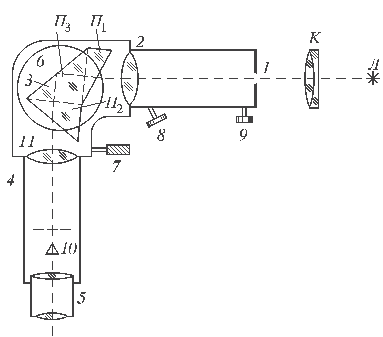
\includegraphics[scale=1]{ustanovka1.pdf}{\label{pic1}}}
				\ffigbox[\FBwidth]{\caption{}}%
				{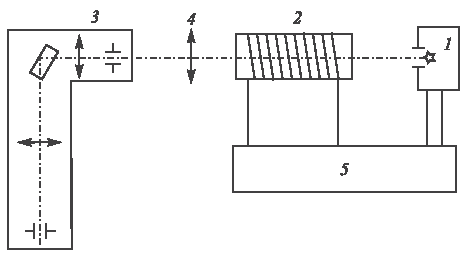
\includegraphics[scale=1]{ustanovka2.pdf}{\label{pic2}}}         
			\end{subfloatrow}
		}
		{\caption{Экспериментальная установка.}}
	\end{figure}
	
	В нашей работе спектр поглощения паров йода наблюдается визуально на фоне сплошного спектра лампы накаливания 1, питаемой от блока питания 2 (рис.~\ref{pic2}).
	
	\newpage
	\section{Экспериментальные данные}
	
		\floatsetup[table]{capposition=top}	
		\begin{table}[H]
			\caption{Каллибровка спектрометра.}
			\label{table:exp}
			\begin{tabular}{|c|c|c|}
				\hline
				$\theta$, дел. & $\sigma_\theta$, дел. & $\lambda$, нм \\ \hline
				6717           & \multirow{28}{*}{1}   & 2558          \\ \cline{1-1} \cline{3-3} 
				6678           &                       & 2542          \\ \cline{1-1} \cline{3-3} 
				6599           &                       & 2516          \\ \cline{1-1} \cline{3-3} 
				6533           &                       & 2494          \\ \cline{1-1} \cline{3-3} 
				6507           &                       & 2482          \\ \cline{1-1} \cline{3-3} 
				6402           &                       & 2450          \\ \cline{1-1} \cline{3-3} 
				6383           &                       & 2438          \\ \cline{1-1} \cline{3-3} 
				6334           &                       & 2422          \\ \cline{1-1} \cline{3-3} 
				6305           &                       & 2410          \\ \cline{1-1} \cline{3-3} 
				6267           &                       & 2396          \\ \cline{1-1} \cline{3-3} 
				6234           &                       & 2374          \\ \cline{1-1} \cline{3-3} 
				6217           &                       & 2372          \\ \cline{1-1} \cline{3-3} 
				6164           &                       & 2350          \\ \cline{1-1} \cline{3-3} 
				6143           &                       & 2340          \\ \cline{1-1} \cline{3-3} 
				6096           &                       & 2322          \\ \cline{1-1} \cline{3-3} 
				6074           &                       & 2310          \\ \cline{1-1} \cline{3-3} 
				6030           &                       & 2290          \\ \cline{1-1} \cline{3-3} 
				5976           &                       & 2266          \\ \cline{1-1} \cline{3-3} 
				5945           &                       & 2246          \\ \cline{1-1} \cline{3-3} 
				5882           &                       & 2222          \\ \cline{1-1} \cline{3-3} 
				5852           &                       & 2204          \\ \cline{1-1} \cline{3-3} 
				5791           &                       & 2176          \\ \cline{1-1} \cline{3-3} 
				5770           &                       & 2164          \\ \cline{1-1} \cline{3-3} 
				5461           &                       & 1986          \\ \cline{1-1} \cline{3-3} 
				5401           &                       & 1944          \\ \cline{1-1} \cline{3-3} 
				4916           &                       & 1558          \\ \cline{1-1} \cline{3-3} 
				4358           &                       & 896           \\ \cline{1-1} \cline{3-3} 
				4047           &                       & 340           \\ \hline
			\end{tabular}
		\end{table}
	
	\newpage
	\section{Обработка результатов}
		Проградуируем спектрометр, для чего используем спектры неоновой и ртутной лампы, длины волн спектральных линий которых известны. Результаты измерений представлены в таблице~\ref{table:exp}.
		\begin{figure}[h!]
			\begin{floatrow}
				\ffigbox[\FBwidth]{\caption{Каллибровка спектрометра.}\label{fig:callibr}}%
				{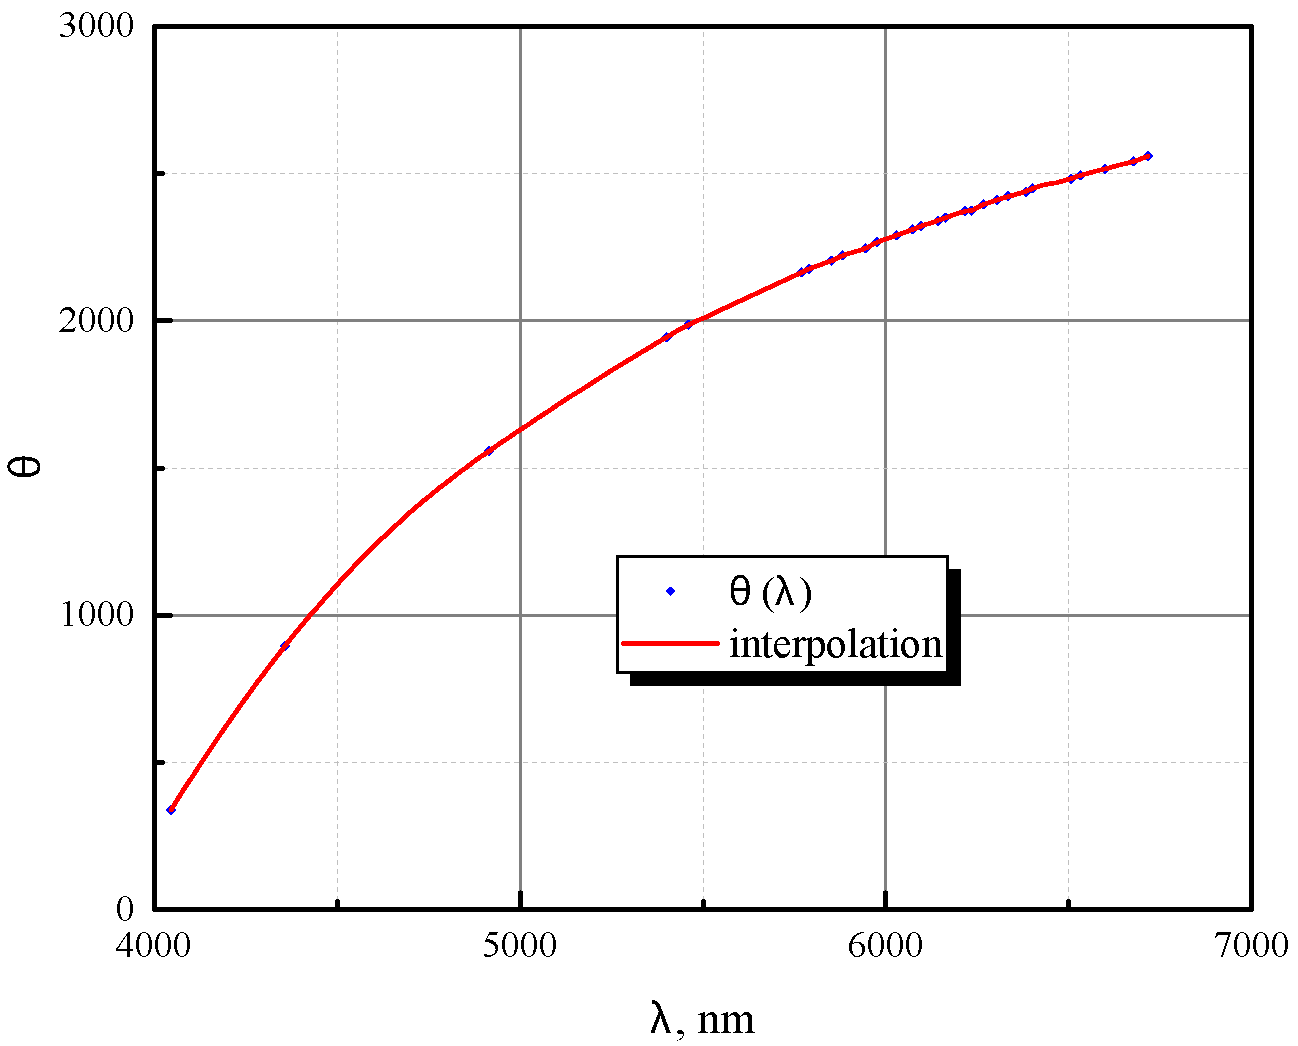
\includegraphics[scale=0.5]{graph.pdf}}
			\end{floatrow}
		\end{figure}
	
		Для интерполяции графика (\ref{fig:callibr}) на все промежуточные значения используем формулу Гартмана:
		\begin{equation*}
			\lambda=\lambda_0+\dfrac{C_0}{\theta-\theta_0},
		\end{equation*}
		где $\lambda_0, C_0,\theta_0$ суть параметры, определяемые по трём ближайшим точкам графика.
		
		Измерим положения трёх линий водорода из серии Бальмера --- $H_{\alpha}, H_{\beta}, H_{\gamma}$. Линию $H_{\delta}$ пронаблюдать не удалось ввиду её слабой интенсивности.	Получили соответствующие показания спектрометра:
		\begin{equation*}
			H_{\alpha}: 2500\pm 1, \  H_{\beta} : 1508 \pm 1, \ H_{\gamma} : 874 \pm 1.
		\end{equation*}
		С учётом градуировки спектрометра получаем следующие длины волн: 
		\begin{equation*}
			H_{\alpha} = 656 \pm 2 \ \text{нм}, \ H_{\beta} = 487 \pm 2 \ \text{нм}, \ H_{\gamma} = 434 \pm 2\  \text{нм}.
		\end{equation*}
		
		
		Для каждой линии определим константу Ридберга по формуле (\ref{eq:Ry}), учитывая, что $m=2$, $Z=1$, а также, что для линии $H_{\alpha}$ --- $n=3$, для линии $H_{\beta}$ --- $n=4$, для линии $H_{\gamma}$ --- $n=5$. Получаем следующие значения константы Ридберга:
		\begin{equation*}
			\text{Ry}_{\alpha}=(0.0110 \pm 0.0001) \ \text{нм}^{-1}, \ \text{Ry}_{\beta} =( 0.0109 \pm 0.0001)\ \text{нм}^{-1}, \ \text{Ry}_{\gamma}=(0.0109 \pm 0.0001) \ \text{нм}^{-1}.
		\end{equation*}
	
		По МНК определяем наилучшее значение константы Ридберга, а также его погрешность:
		\[\boxed{\text{Ry}_E=(0.0109\pm 0.0002) \ \text{нм}^{-1}}\]
		Полученное значение в пределах погрешности совпадает с табличным значением: $$\text{Ry}=0.01097 \ \text{нм}^{-1}.$$
		
		Запишем показания спектрометра для следующих переходов в молекуле йода: $\theta_{1,0}$ -- переход из первого колебательного уровня основного состояния в нулевой колебательный уровень возбуждённого состояния,  $\theta_{1,5}$ -- переход из первого колебательного уровня основного состояния в пятый колебательный уровень возбуждённого состояния, $\theta_{g}$ -- переход из нулевого колебательного уровня основного состояния в область непрерывного спектра возбуждённого состояния. Получаем следующие данные:
		\begin{equation*}
			\theta_{1,0}=2344 \pm 1, \ \theta_{1,5}=2242 \pm 1, \ \theta_g=1850 \pm 1,
		\end{equation*}
		 откуда находим соответствующие длины волн: 
		 \begin{equation*}
		 	\lambda_{1,0}=(615 \pm 2) \ \text{нм}, \ \lambda_{1,5}=(594 \pm 2) \ \text{нм}, \ \lambda_g=(522 \pm 2)\ \text{нм}.
		 \end{equation*}
		
		Определим энергию колебательного кванта возбуждённого состояния молекулы по формуле: 
		\begin{equation*}
			h \nu_2=\dfrac{h\nu_{1,5}-h \nu_{0,5}}{5}.
		\end{equation*}
		Итого:
		\begin{equation*}
			h\nu_2=(0.014\pm 0.002) \ \text{эВ}
		\end{equation*}
			
		Вычислим энергию электронного перехода $\Delta E=E_2-E_1$, энергию диссоциации $D_1$ в основном состоянии и энергию диссоциации $D_2$ в возбуждённом состоянии, если известно, что энергия колебательного кванта основного состояния есть $h\nu_1=0,027$~эВ, а энергия возбуждения, то есть энергия перехода атома из области непрерывного спектра основного состояния в область непрерывного спектра возбуждённого состояния, равна $E_A=0.94$ эВ.\\
		Имеем систему уравнений:
		\begin{equation*}
			\begin{cases}
				D_1+E_A=h \nu_g,\\
				h\nu_g=D_2+\Delta E,\\
				h\nu_{1,0}=\Delta E+h\nu_2-\dfrac{3}{2}h\nu_1,\\
					h\nu_{1,5}=\Delta E+\dfrac{11}{2}h\nu_2-\dfrac{3}{2}h\nu_1.
			\end{cases}
		\end{equation*}

		Из неё находим все необходимые величины:
		\[\boxed{\Delta E=(2.050\pm 0.002) \ \text{эВ}, \ D_1=(1.436\pm 0.002)\  \text{эВ}, \  D_2=(0.326 \pm 0.002) \ \text{эВ}.}\]

\section{Обсуждение результатов и выводы}
	В работе исследовались сериальные закономерности в оптическом спектре водорода и спектр поглощения паров йода в видимой области.
	
	С помощью информации о спектральных линиях неона и ртути проградуирован спектрометр. Построен соответствующий график.
	
	Получены длины волн линий $H_{\alpha}$, $H_{\beta}$ и $H_{\gamma}$ серии Бальмера, вычислена постоянная Ридберга. В рамках погрешности данные совпали с табличными.
	
	Получены длины волн, соответствующие некоторым электронно-колебательным переходам из основного состояния в возбуждённое. Вычислены энергия колебательного кванта возбуждённого состояния молекулы, энергия электронного перехода, энергии диссоциации молекулы в основном и в возбуждённом состояниях.


\end{document}